\documentclass[a4wide]{report}

\usepackage{amsmath}
\usepackage[a4paper, total={7in, 10.2in}]{geometry}
\usepackage{graphicx}
\usepackage[portuguese]{babel}
\usepackage[utf8]{inputenc}


\begin{document}

\noindent
{\bf Rafael V. Cacilhas  - Relatório 04 (\today)}

\vspace{0.5cm}

\section*{Exercício 1}

\subsection*{a) }

Calcularemos todas as constantes no SI. Assim:


\begin{equation*}
D= \frac{k_b T}{6 \pi \eta a} \approx 2.923 \times 10^{-9} \frac{m^2}{s}
\end{equation*}

\begin{equation*}
\Delta t = \frac{\lambda h^2}{D} 
\end{equation*}
\begin{equation*}
\Delta t = \frac{0.1  \left( 5 \times 10 ^{-4} \right) ^2 }{2.923 \times 10^{-9} } = 8.55 s
\end{equation*}

No programa não foi utilizado o sistema de unidades SI. Nele, temos $D = 0.2923  \mu m^2/ms$ e, por consequencia, $\Delta t = 8.55 \times 10^{-4}s$, de modo a manter $\lambda = 0.1$. Na Figura \ref{1} temos um gráfico da concentração em função da posição para diferentes tempos t (em segundos).

\begin{figure}[!htb]
\centering
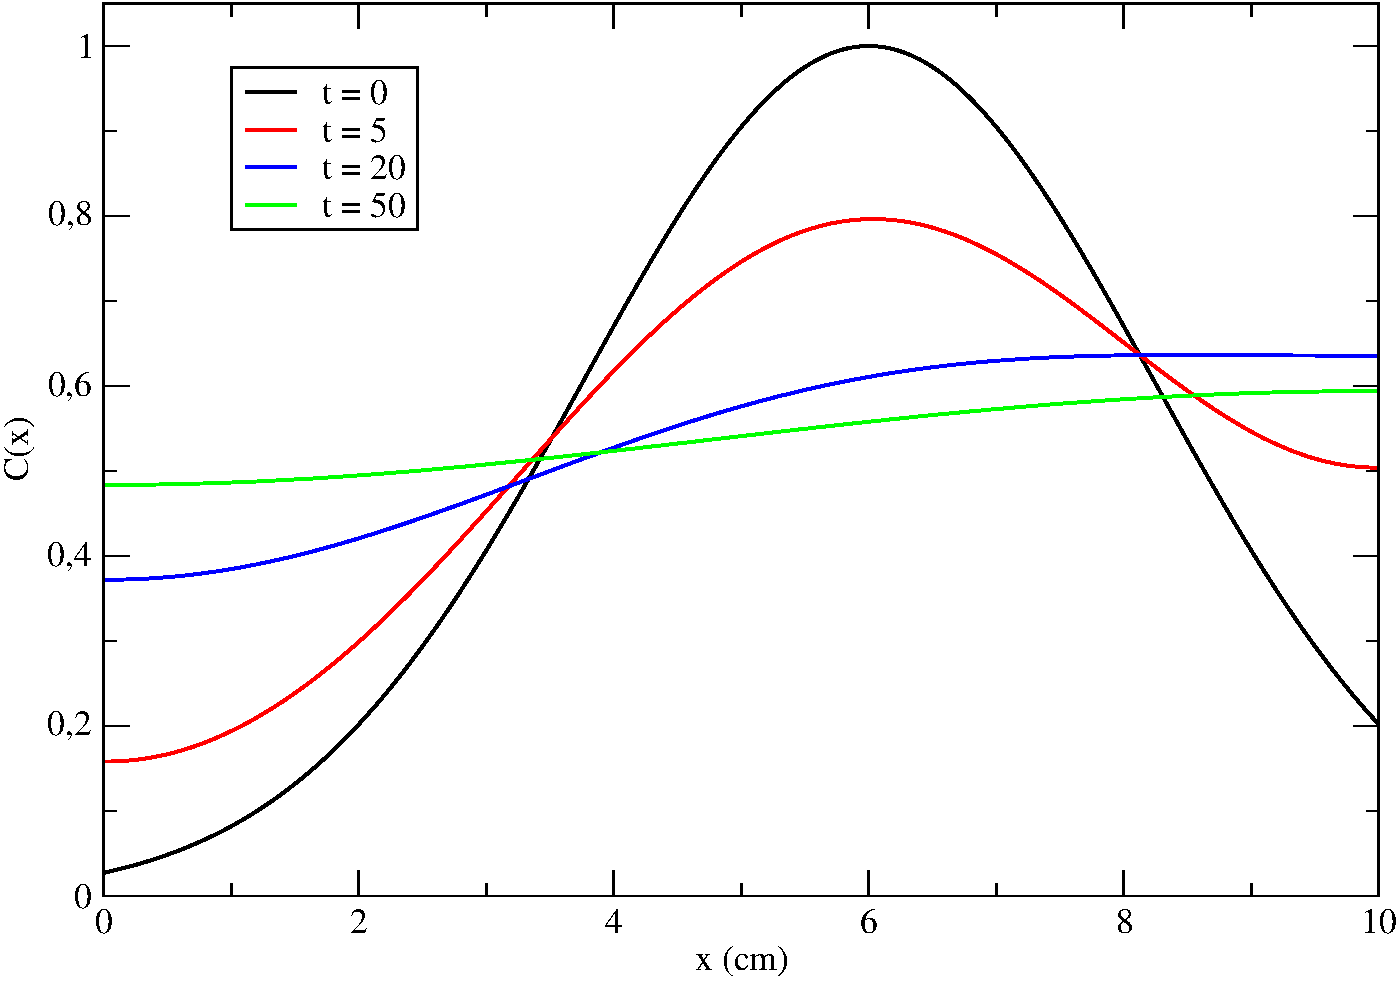
\includegraphics[width=0.447\textwidth]{c.pdf}
\caption{Concentração em função da distância para diferentes tempos.}
\label{1}
\end{figure}

É possivel notar que a medida que o tempo passa a distribuição inicialmente gaussiana passa a assumir uma forma cada vez mais constante, como era esperado. Para $t = 50s$ temos que a concentração varia apenas entre aproximadamente 0.48 e 0.6, apresentando uma solução quase homogênea.


\section*{Exercício 2}

\subsection*{a)}

Expandindo $V(x,y)$ em sua série de Taylor temos que:


\begin{equation}
V(x + h,y) = V(x,y) + h \frac{\partial V}{\partial x} + \frac{h^2}{2} \frac{\partial^2 V}{\partial x^2} + O(h^3) 
\end{equation}

\begin{equation}
V(x - h,y) = V(x,y) - h \frac{\partial V}{\partial x} + \frac{h^2}{2} \frac{\partial^2 V}{\partial x^2} + O(h^3) 
\end{equation}

\begin{equation}
V(x,y+h) = V(x,y) + h \frac{\partial V}{\partial y} + \frac{h^2}{2} \frac{\partial^2 V}{\partial y^2} + O(h^3) 
\end{equation}

\begin{equation}
V(x,y-h) = V(x,y) - h \frac{\partial V}{\partial y} + \frac{h^2}{2} \frac{\partial^2 V}{\partial y^2} + O(h^3) 
\end{equation}

Somando as quatro equações acima, temos:

\begin{equation*}
V(x + h,y) + V(x-h,y) + V(x,y+h) + V(x,y-h) = 4 V(x,y) + O(h^2) 
\end{equation*}

E, portanto:

\begin{equation}
 V(x,y) = \frac{ V(x + h,y) + V(x-h,y) + V(x,y+h) + V(x,y-h)}{4}
\end{equation}


\subsection*{b)}
A subrotina está implementada no programa laplaceB.f90 

\subsection*{c)}
Na Figura \ref{2c} temos a solução para V(x,y) no fio quadrado. Utilizamos um mapa de cores para representar as voltagens em cada ponto (x,y) utilizando o \textit{gnuplot}. Idealmente esta imagem não apresentaria este quadriculado (oriundo das discretizações), teria uma fonte maior na escala e teria uma proporção de 1:1, mas não soube fazer estas configurações no gnuplot. O gráfico, portanto, foi feito com as configurações padrões do \textit{gnuplot}.
\begin{figure}[!htb]
\centering
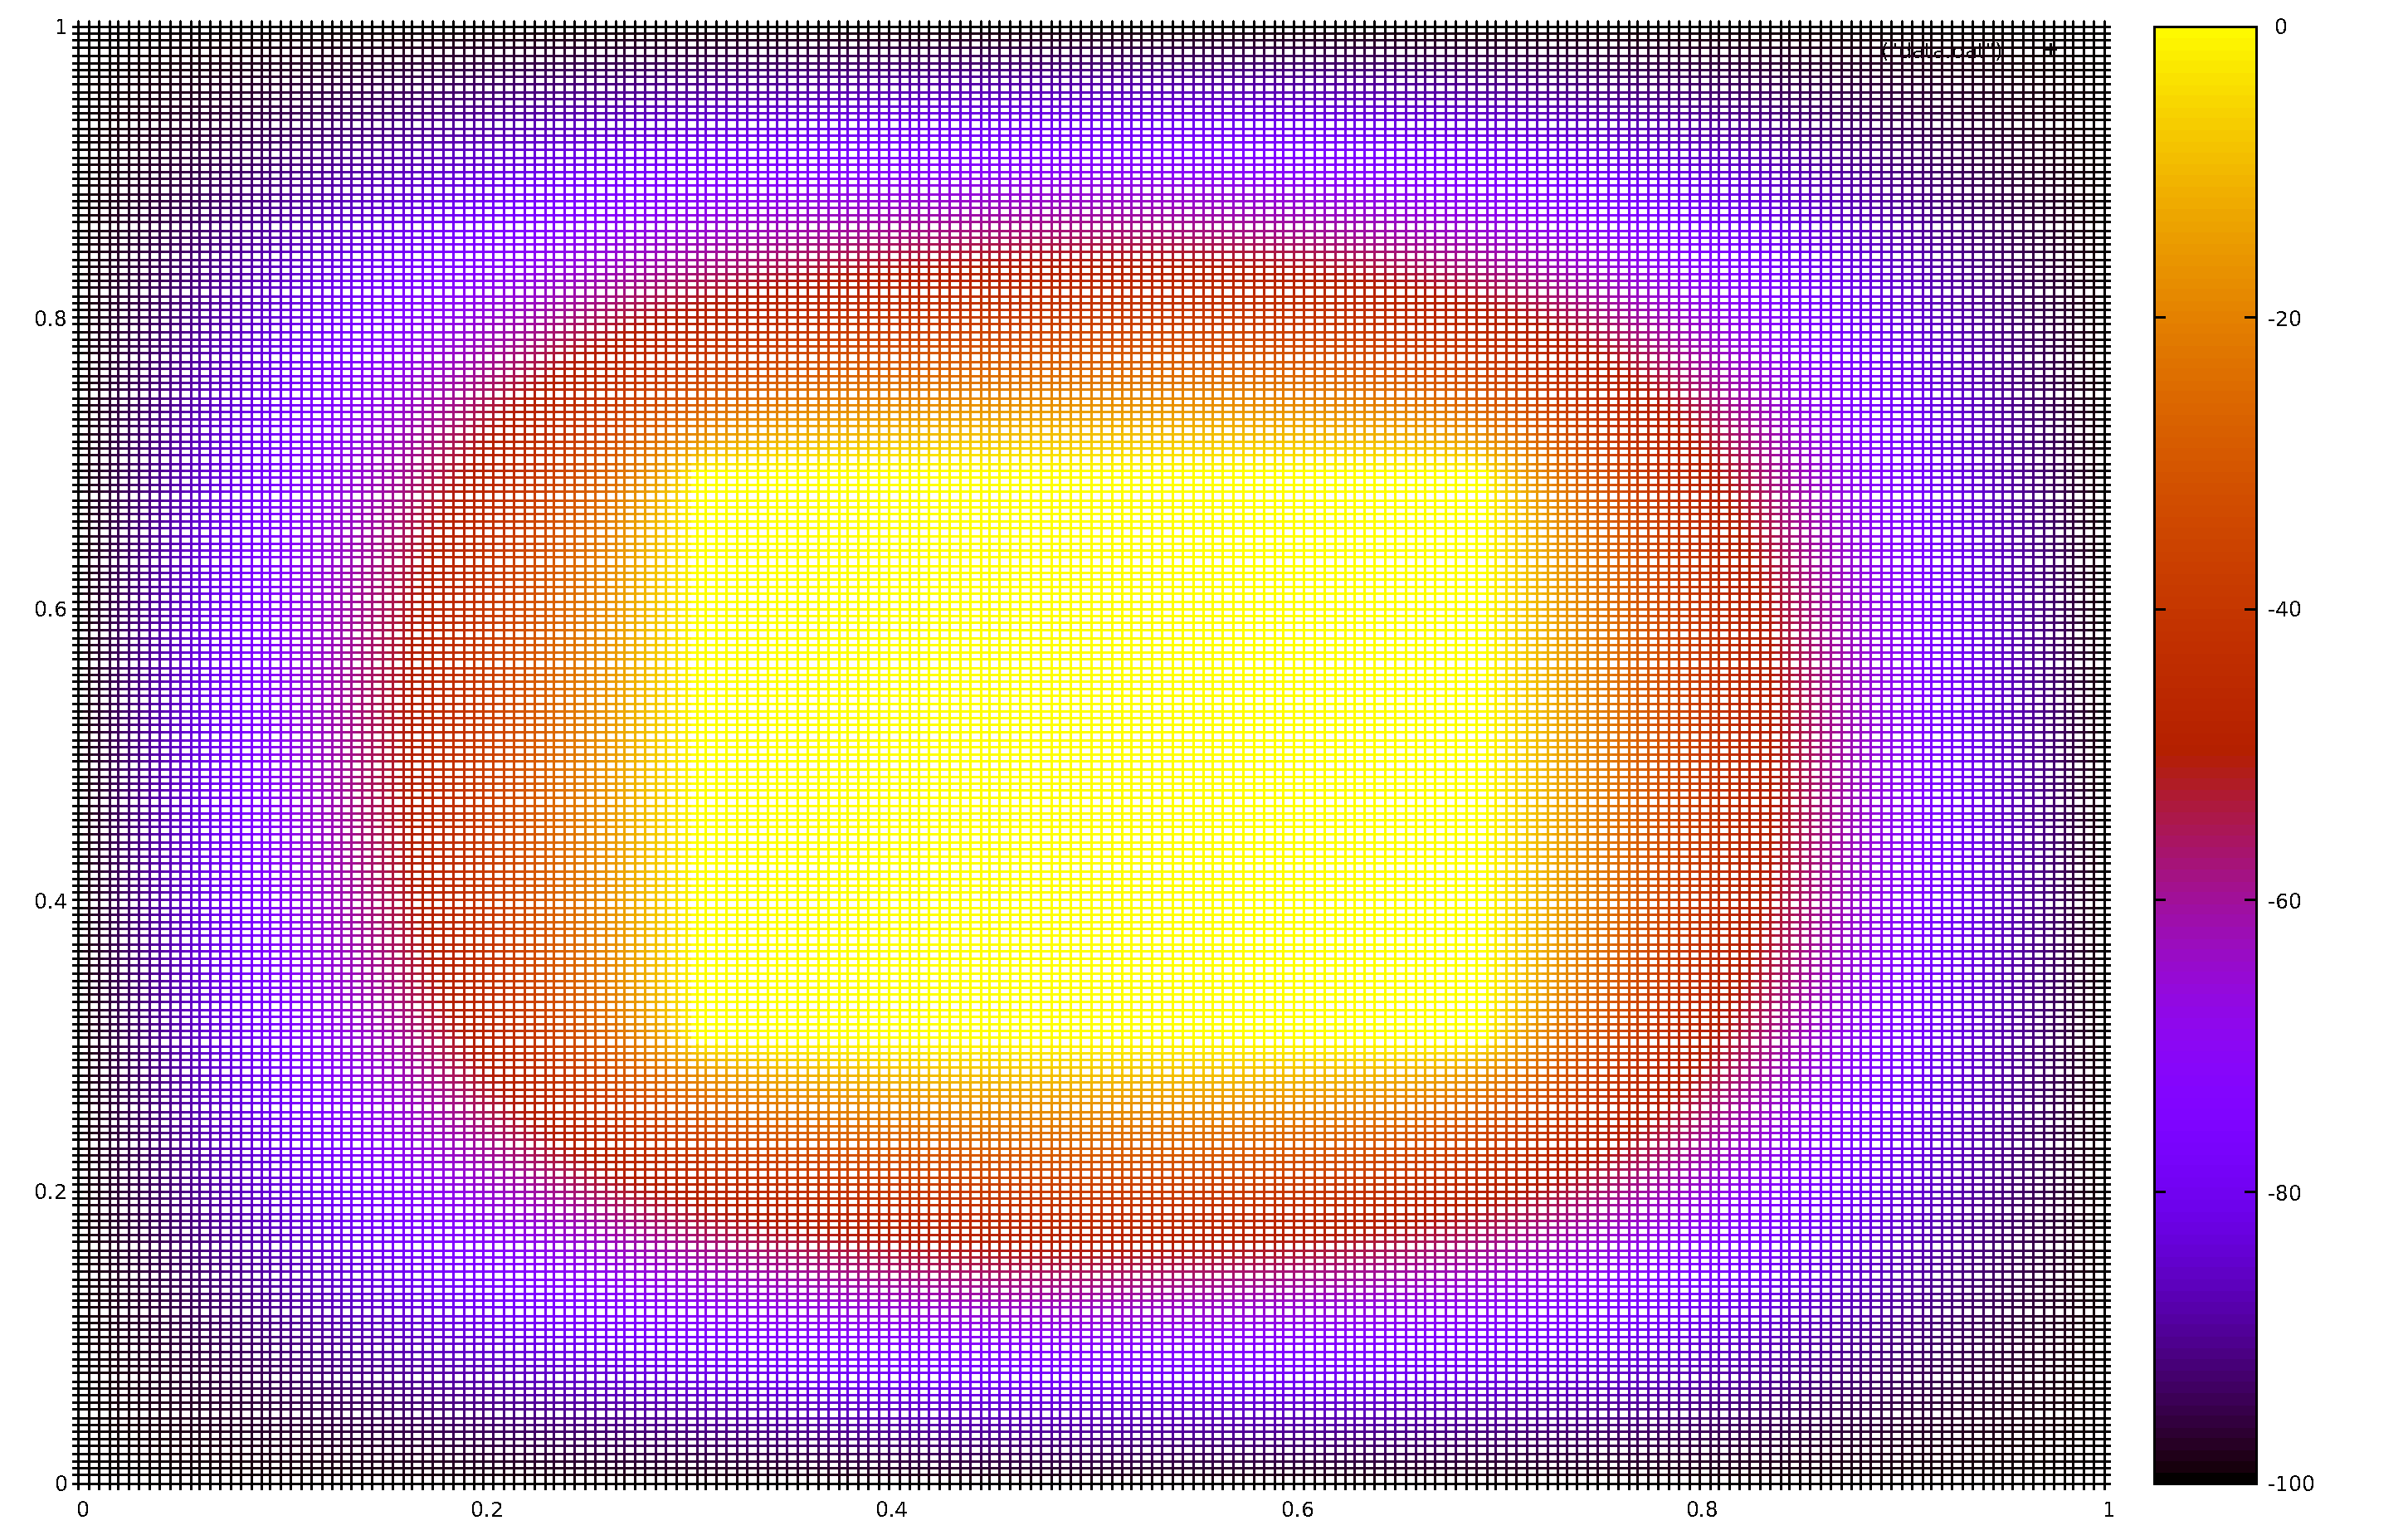
\includegraphics[width=0.447\textwidth]{2.pdf}
\caption{Solução da equação de Laplace para o fio quadrado.}
\label{2c}
\end{figure}



\section*{Exercício 3}
\subsection*{a)}
Primeiramente é preciso notar que o exercício possui erros de lógica na sua formulação. É incoerente exigir que $\begin{cases} 
i(x,0) = 5.5 \cos\left( \frac{\pi }{200}x \right) \\
i(0,t) = i(200,t) = 0
\end{cases} $
sejam satisfeitas simultaneamente. Para resolver isto temos duas soluções: podemos acrescentar uma fase a $i(x,0)$ ou exigir que $i(0,t) = -i(200,t) = 5.5$. Vamos escolher o último caso, pois assim a corrente e a voltagem ficam fora de fase para todos os pontos. Assim sendo, queremos resolver a EDP:

\begin{equation*}
\frac{\partial^2 V}{\partial x^2} = LC \frac{\partial^2 V}{\partial t^2}
\end{equation*}
\begin{equation*}
\frac{\partial^2 i}{\partial x^2} = LC \frac{\partial^2 i}{\partial t^2}
\end{equation*}

sob as seguintes condições:

\begin{equation*}
0 \leq x \leq 200
\end{equation*}
\begin{equation*}
L = 0.3 henries/ft
\end{equation*}
\begin{equation*}
C = 0.1 farads/ft
\end{equation*}
\begin{equation*}
V(0,t) = V(200,t) = 0
\end{equation*}
\begin{equation*}
V(x,0) = 110 \sin \left(\frac{\pi}{200} x\right)
\end{equation*}
\begin{equation*}
\frac{\partial V(x,0)}{\partial t} = 0
\end{equation*}
\begin{equation*}
i(0,t) = -i(200,t) = 5.5
\end{equation*}
\begin{equation*}
i(x,0) = 5.5 \cos \left(\frac{\pi}{200} x\right)
\end{equation*}

\begin{equation*}
\frac{\partial i(x,0)}{\partial t} = 0
\end{equation*}

Neste caso a situação inicial está representada na Figura \ref{3a}.

\begin{figure}[!htb]
\centering
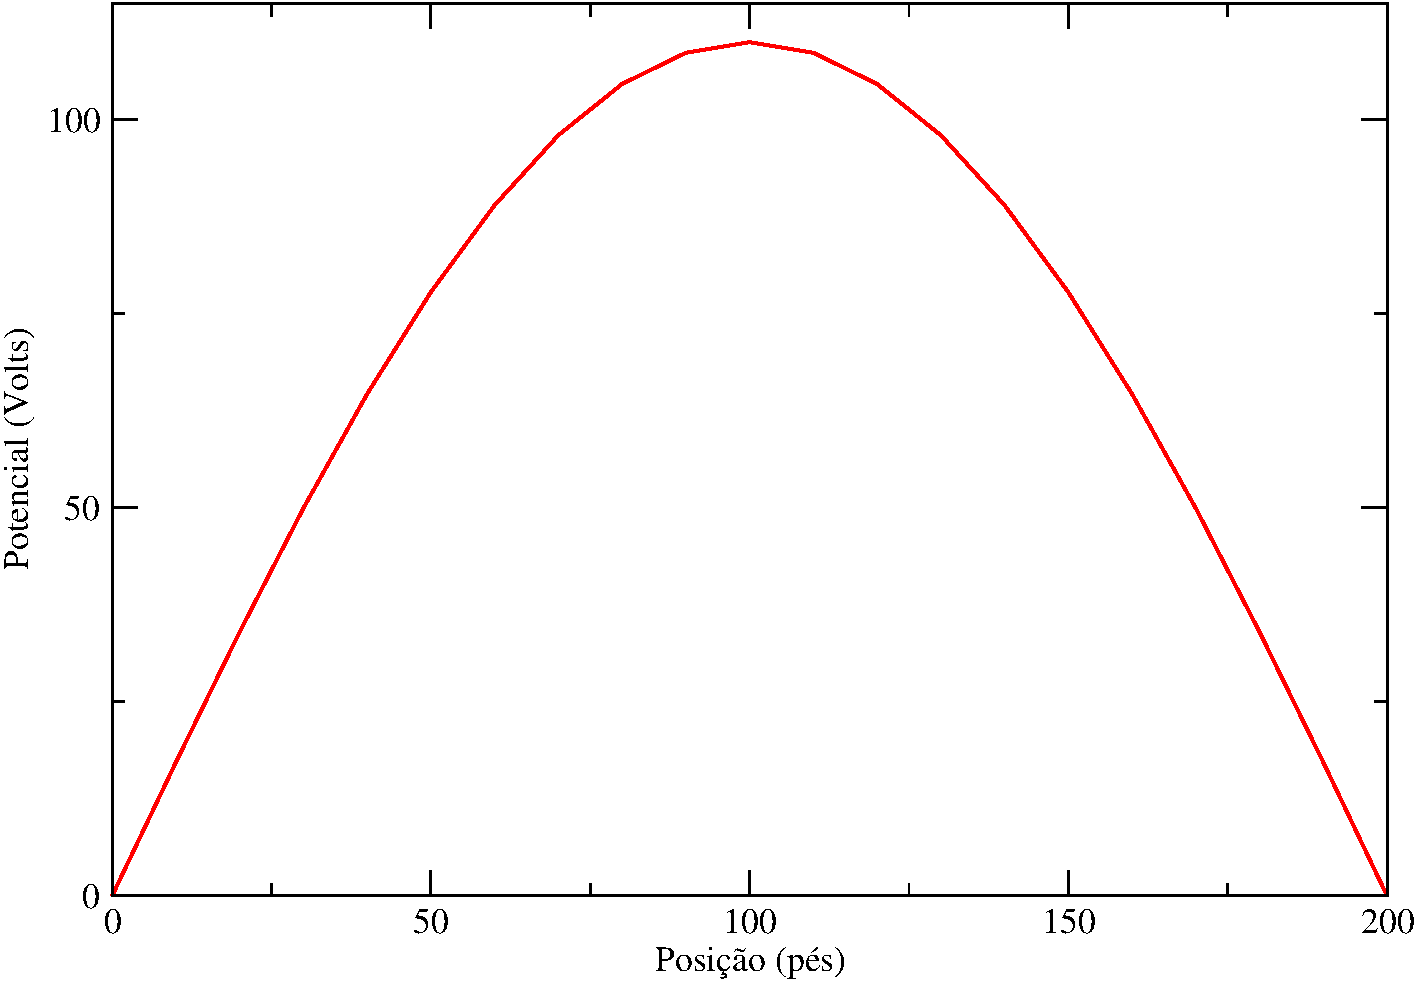
\includegraphics[width=0.447\textwidth]{V0.pdf}
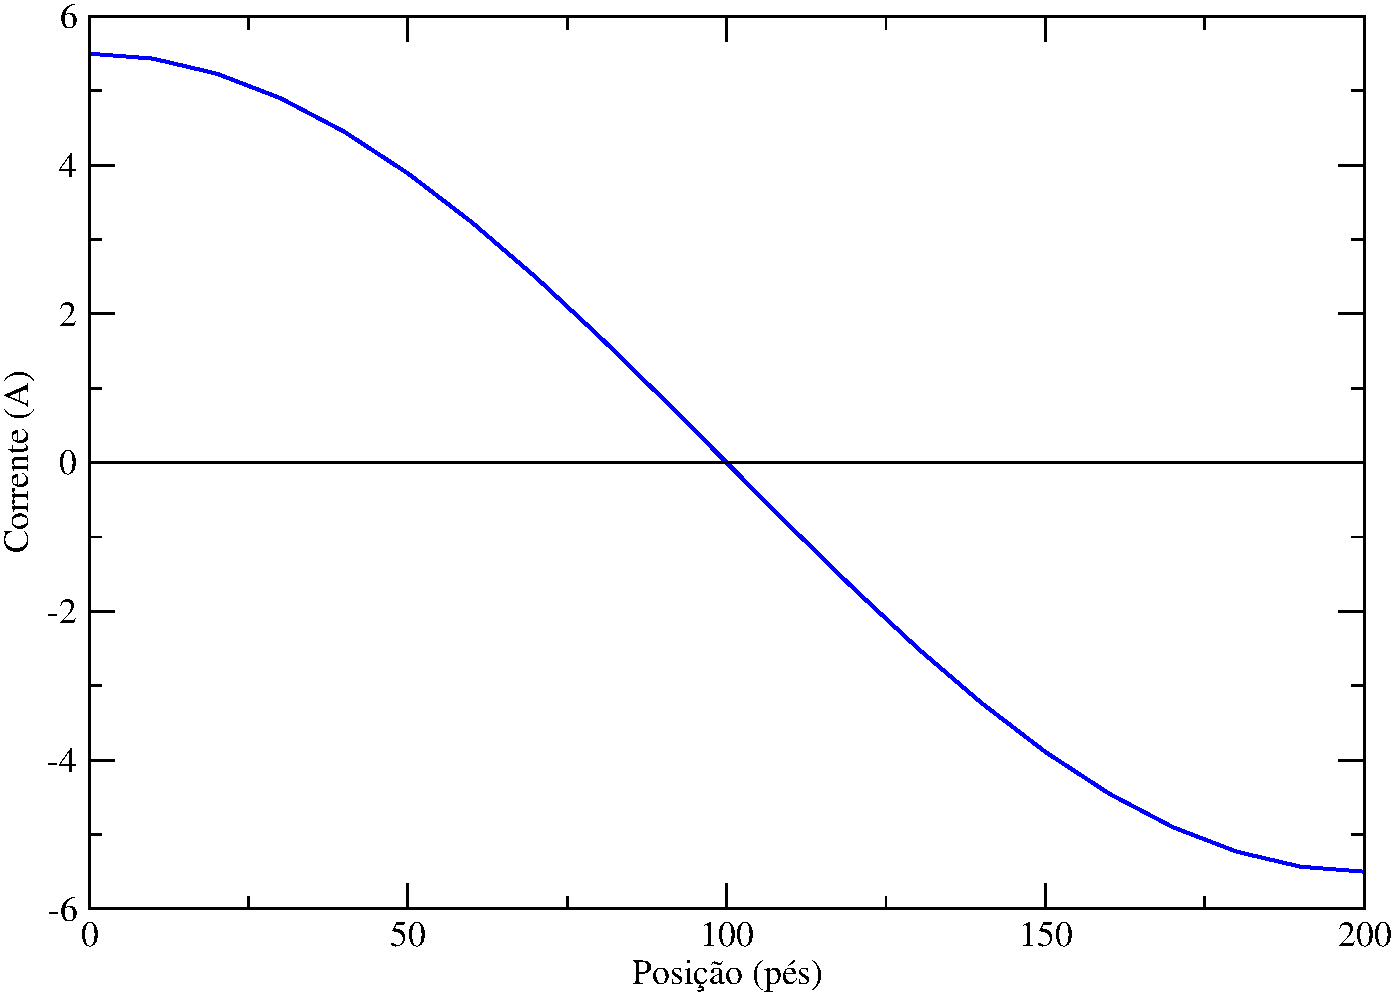
\includegraphics[width=0.447\textwidth]{i0.pdf}
\caption{Voltagem (esquerda) e corrente (direita) inicial.}
\label{3a}
\end{figure}

Para o tempo t = 0.2 a solução está na Figura \ref{3b}.

\begin{figure}[!htb]
\centering
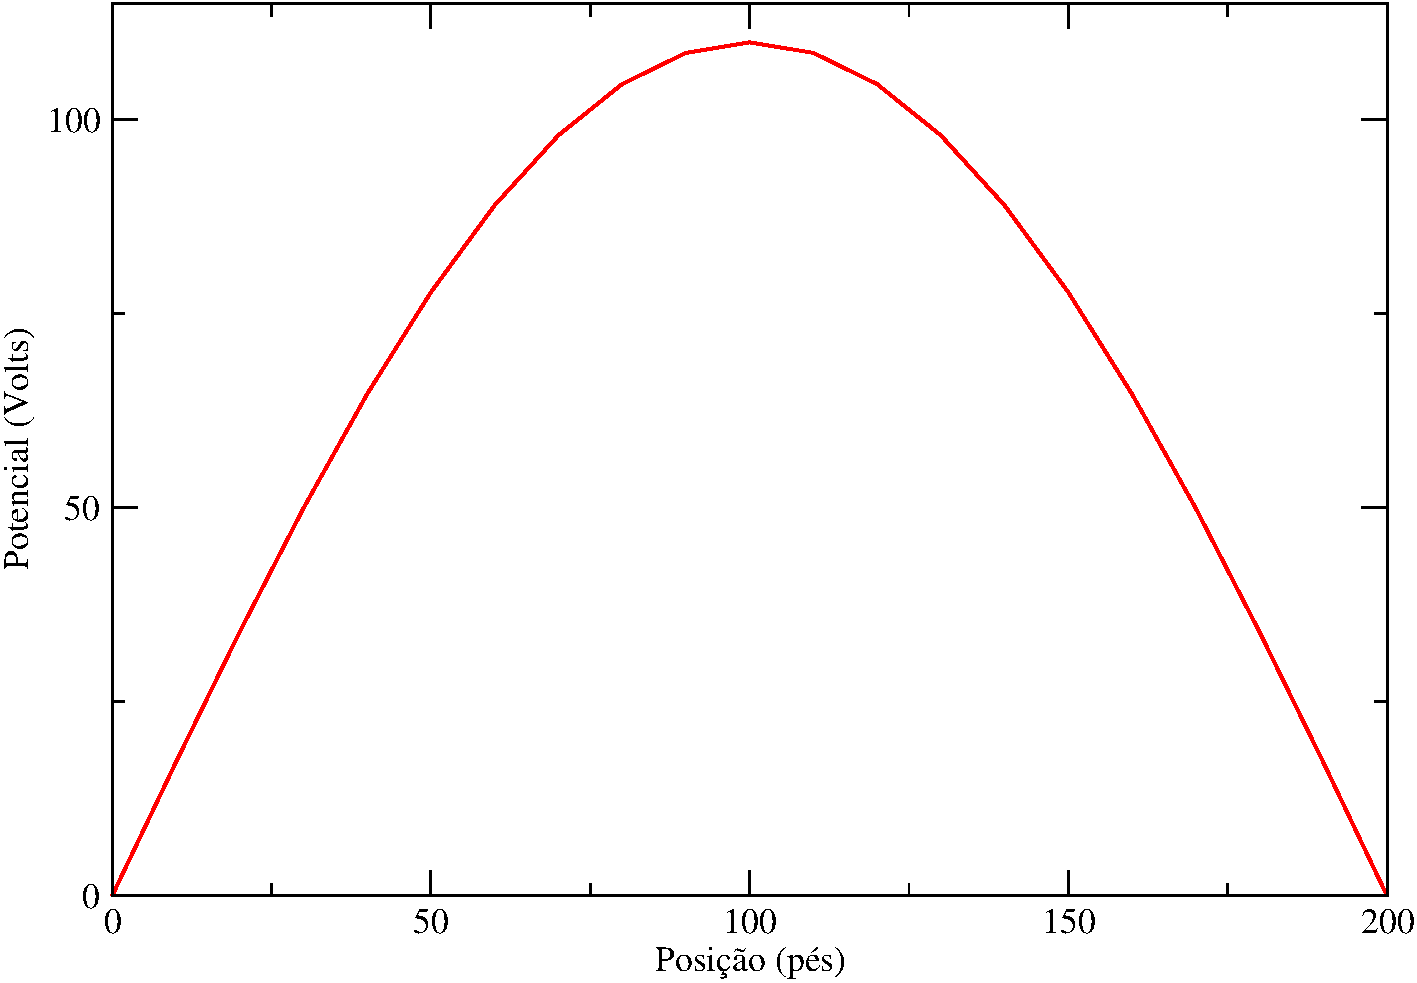
\includegraphics[width=0.447\textwidth]{V2.pdf}
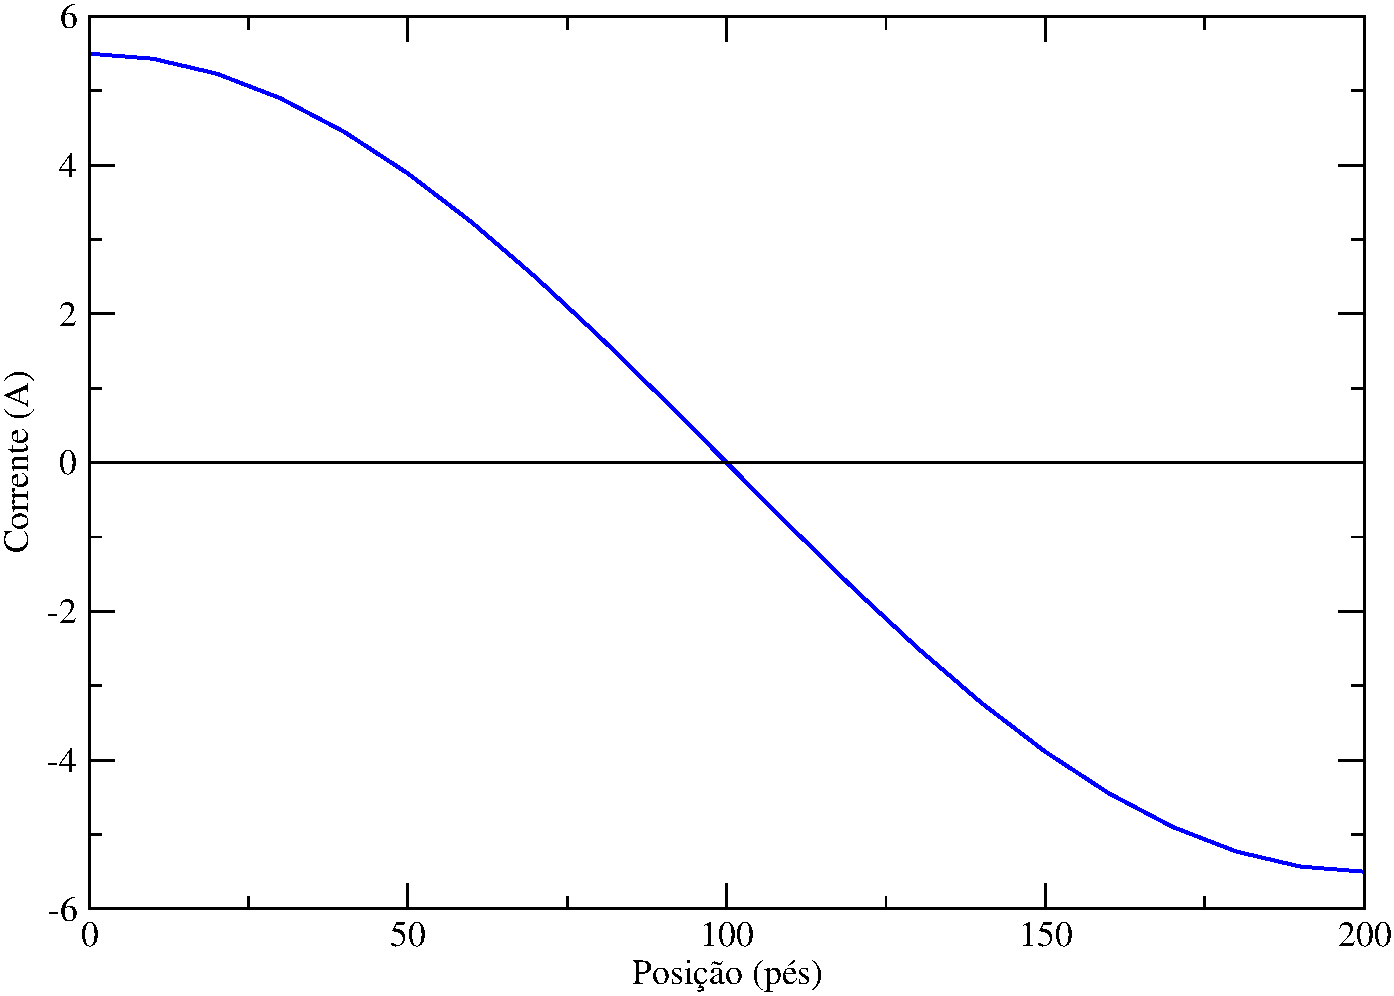
\includegraphics[width=0.447\textwidth]{i2.pdf}
\caption{Voltagem (esquerda) e corrente (direita) para o tempo t = 0.2.}
\label{3b}
\end{figure}

Para o tempo t = 0.5 a solução está na Figura \ref{3c}.

\begin{figure}[!htb]
\centering
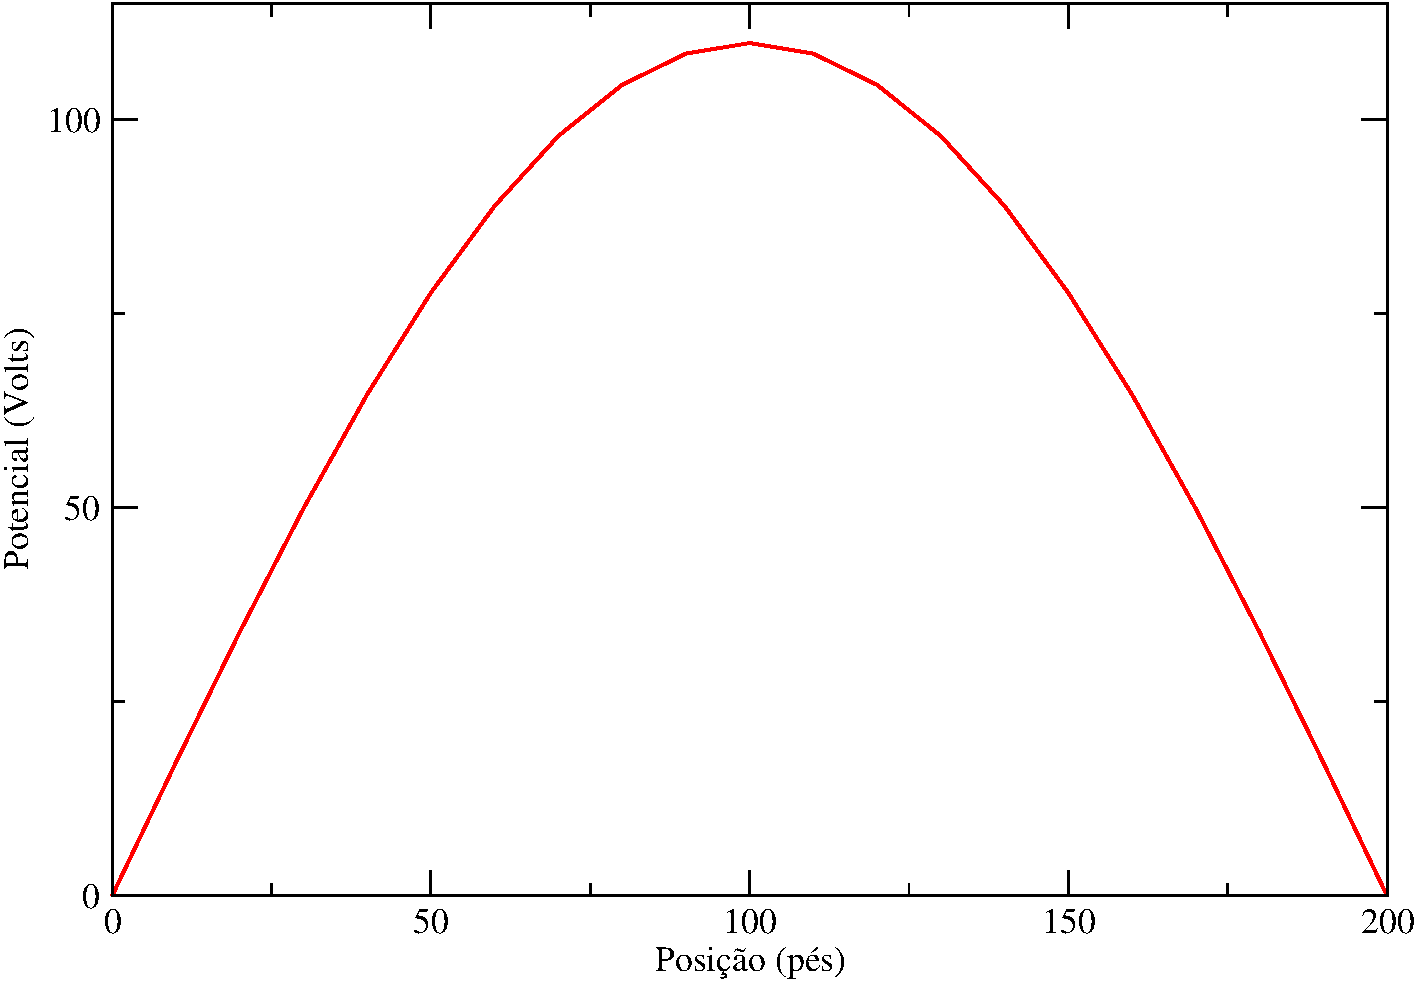
\includegraphics[width=0.447\textwidth]{V5.pdf}
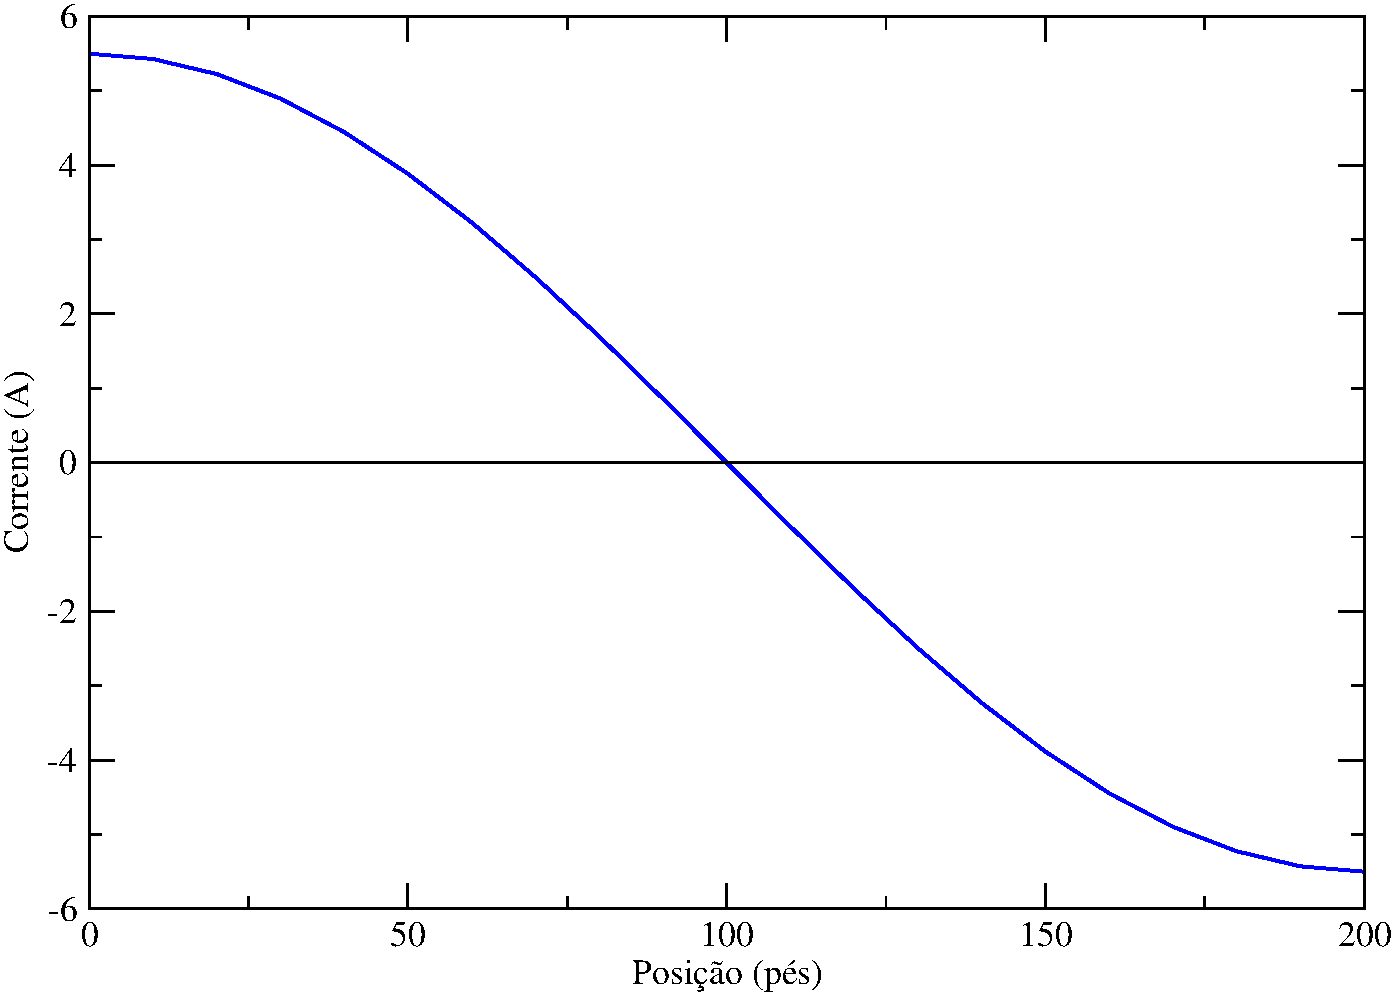
\includegraphics[width=0.447\textwidth]{i5.pdf}
\caption{Voltagem (esquerda) e corrente (direita) para o tempo t = 0.5.}
\label{3c}
\end{figure}

Não é possível observar nenhuma mudança entre os três tempos diferentes apresentados. Isto se deve ao fato de que esse sistema oscila com uma frequência angular dada por $\omega = \frac{1}{\sqrt{LC}} \approx 1.76 Hz$. Assim, a frequência de oscilação é $ f \approx 0.28 Hz$ e de fato uma mudança significativa demoraria alguns poucos segundos para acontecer.

\end{document}
